\documentclass{scutmaster}

\usepackage{graphicx}
\usepackage{hyperref}
\usepackage{xcolor}

\DeclareMathOperator*{\argmax}{arg\,max}
\DeclareMathOperator*{\argmin}{arg\,min}

\newcommand{\TODO}[1]{\textcolor{red}{TODO: #1}}

\title{基于可微分渲染的人脸3D重建}
\titleEN{Face 3D Reconstruction Based on Differentiable Rendering}
\classificationnumber{TP37}

\author{胡玮文}
\authorEN{Weiwen Hu}
\studentnumber{202045611}
\phone{17701952145}
\email{sehuww@mail.scut.edu.cn}
\address{江西省南昌市青山湖区江大南路139号荣昌小区16栋(330029)}

\degree{工学硕士}
\major{软件工程}{数字人}

\supervisor{杜卿}{副教授}
\supervisorEN{Assoc. Prof.}{Qing Du}

\school{软件学院}

\begin{document}

\maketitle
\maketitleEN
\nominationpage
\declareoforiginality

\frontmatter
\chapter{摘要}

你好,世界!

\keyword{关键词} 可微分渲染

\chapter{Abstract}

Hello, world!

\keyword{Keywords} Differentiable rendering

\tableofcontents

\listoffigures

\mainmatter
\chapter{绪论}
\label{chap:intro}

\section{研究背景}

3D人脸重建是计算机视觉和计算机图形学领域的一个热门研究方向。
相比于传统计算机视觉对2D照片的判断、识别和生成,3D人脸表示更加贴近实际,并可以建模光照和视角产生的影响。
例如,3D人脸模型可显式地表达人脸在3D空间中的位置,姿态甚至表情和骨骼的位置;
高质量的模型可用于逼真地一致地渲染出不同环境和视角下的人脸图像。

但相比于普通的摄影,3D人脸模型带来的优势是以更复杂的捕获过程为代价的,这通常会限制其应用范围。
直接捕获3D人脸信息通常需要立体视觉系统\citep{DEP,ss_geo}、3D激光扫描仪(如NextEngine和Cyberware)或RGB-D相机\citep{li2023}(如Kinect)。
前两种能捕获高质量的人脸扫描,但需要受控环境和昂贵的机器。
相比之下,RGB-D相机更便宜,更易于使用,但所得到的扫描质量有限。

在计算机图形学领域,
高质量的人脸模型已经可以用于在计算机中忠实地重现人脸,
包括角质层的凹凸、毛孔、皱纹、镜面反射和次表面散射等复杂特性。
这些模型已经在影视、游戏、动画、虚拟现实等领域中广泛应用,
但是其获取成本非常高昂。
目前成熟的影视级3D人脸重建方案仍是昂贵的商业解决方案,
其中包括大量复杂的步骤,并需要大量美术和技术人员参与制作\footnote{https://blog.unity.com/technology/making-of-the-heretic-digital-human-character-gawain}。
这些高精度重建方案通常使用专用设备在受控环境扫描的精细数据。
它们基于专业的摄影设备和完全受控的数据处理流程,
通过摄影测量的方法,使用相机作为测量仪器精确定量地测定各个方向上光线强度。
并基于较为准确的光学模型重建人脸的几何和材质。

相比之下,能从普通非受限环境的照片或视频中重建3D人脸模型的高效重建方法受到了广泛关注。
这类方法只需要最少单张手机随意拍摄的照片即可实时完成3D重建。
它结合了2D图像拍摄的便捷性和3D人脸模型的优势,
其应用非常广泛,目前已被用于人脸识别\citep{BlanzV03,1022631413.nh,zhu2015high}、人脸表情捕捉\cite{Mo2022TowardsAF}、人脸跟踪\citep{Pham2016RobustRP}、人脸动画合成\citep{Cao20133DSR,thies2016face2face}等任务中,并有代替人脸关键点识别等2D分析方法的潜力。

然而,该任务如今依然非常具有挑战性。
从少量非受限环境中拍摄的照片重建3D模型是高度不适定的。
算法需要从单张照片中估计出人脸几何形状、头部姿势和纹理、环境光照等参数,
参数空间很大,而不同解之间存在歧义,因为同一张照片可以从不同的3D模型中生成,
并且很难确定哪个模型才更加准确。
因此该任务必须结合有关人脸的先验知识才能完成。

基于人脸3D可形变模型(3D Morphable Model,简称3DMM)和神经网络的方法能以数据驱动的方式更好地建模有关人脸的先验知识。
3DMM是从大量人脸3D扫描中得到的统计模型,其先验知识通常编码于均值、方差等统计量中;
而神经网络则能从各种各样的监督信号中学习先验知识,例如3D模型、照片、关键点或高阶的人脸识别特征等。
这些先验知识有助于缓解3D重建的解之间的歧义。
在这些方法的加持下,我们虽然已经能高效地获得较为准确的3D人脸模型,
但这些模型都牺牲了大多数环境以及人脸表面上的细节,无法再次渲染从而忠实地还原照片,
因而并不能直接应用于影视,游戏等工业领域中。
另外,部分监督信号需要较为复杂的额外步骤才能得到,且可能引入额外的误差,
例如人脸关键点检测中,部分关键点的位置不论在照片或是在3D模型上都难以准确定义。
可以预见,在数字孪生和元宇宙等概念走入公众视野的今天,
基于现实的形象批量生产高渲染质量的人脸模型将涌现新的需求,
基于少量非受限环境照片的方便快捷的3D人脸重建技术具有重要现实意义。

在人脸重建方法中,可微分渲染技术已占有一席之地。
该技术旨在准确估计3D渲染结果关于其渲染参数(模型、光照等)的梯度,
从而引入直接的合成分析(Analysis by Synthesis)方法,也即逆渲染方法。
如今从模型渲染图片的过程已十分复杂,且随着计算机图形学和神经渲染等技术的发展还在不断进化,对人脸则更是如此。
而逆渲染方法直接将渲染结果和输入照片进行比较,根据渲染的误差来优化渲染参数,以此适应任意复杂的渲染方式。
可微分渲染则可以支持以简单的梯度下降法实现该优化过程,
具有通用、准确、自动化等优点,可谓是3D模型与2D照片之间的桥梁。
得益于此,基于非受限环境照片的高效重建方法得以直接从大量无标注的人脸照片的数据集中学习3D人脸模型的先验知识。
利用专业采集设备的高精度方案也因此获得更准确的材质参数。

然而,当前可微分渲染在人脸重建领域的应用还非常初步:
在渲染过程的梯度中,由于模型的不同部分之间相互遮挡而产生的可见性梯度通常最为显著,
这些梯度对模型与照片中的边缘的精确对齐至关重要。
但由于渲染采样过程的离散性,这些梯度往往难以估计。
在基于非受限环境照片的方法中,拍摄环境,相机参数,后处理流程等诸多不确定因素更提升了可见性梯度的估计难度。
现有人脸重建方法\citep{BFM,deep3d,DECA,bao2022}均仅考虑了逐像素着色的梯度,忽略了这些难以利用的可见性梯度,
这导致它们未能充分利用照片中的边缘信息,进而无法仅依赖可微分渲染来确定人脸的几何结构。
作为代替,现有方法依赖更加成熟的多目立体(multi-view stereo, MVS)或人脸关键点检测等方法。
但额外步骤将增加重建流程的复杂性,且导致误差在多个环节中累积。

综上,3D人脸重建技术应用广泛。
但现有高精度人脸重建方法所需数据采集环境要求高,实施困难。
在基于非受限环境照片的方法中,对可微分渲染的应用仍有待进一步发展。

\section{本文研究内容及贡献}

本文主要研究3D人脸重建方法的理论与应用。
本文提出了一套高精度多视角数据采集方案,解决了高精度人脸重建所需的数据采集环境要求高,实施困难的问题。
本文从可微分渲染在3D人脸重建中应用时遇到的实际问题出发,
提出了改进的理论,并在实践中验证了其有效性。
本文的主要贡献可概括如下:

\begin{enumerate}
\item 影视级真实的渲染效果离不开基于物理的渲染管线和精确的几何与材质数据。
若要获取这些数据,则需要精确的基于物理的测定。
本文提出了一套多视角人脸数据采集方案,
其旨在通过软硬件协同设计,对全流程的高精度控制,实现在精确的时间点、位置,高分辨率高精度地测定物体反射光线强度数据,
从而为基于物理的可微分渲染的优化提供坚实的基础。
本文介绍了该采集方案的软硬件设计,设备标定校准方法,使用交互方式和实现验证结果。

\item 针对可微分渲染在应用到3D人脸重建时,模型与背景交界处的可见性梯度难以被估计的问题,
本文从理论上分析了其原因是缺乏对背景的建模。
在缺乏对非受限环境中背景的先验知识的前提下,本文提出了面积归一化的像素损失,
以对可微分渲染的损失函数进行改进。
本文通过收缩、扩展两项梯度分析了其作用机理,
并提出了一种几乎无需额外计算和存储开销的方式实现这项改进。
本文通过实验证明了该项改进可以达成既定的目标:
在不对背景建模的情况下,使3D几何模型与照片中的物体边缘良好对齐。

\item 本文实现了一种通过单张在非受限环境中拍摄的照片,重建3D人脸模型的方案。
本文通过集成神经网络和3DMM人脸模型以提升鲁棒性;
通过可微分渲染技术实现更精准的对齐,
并在前述理论的基础上提出了一种基于SDF贴图的方法,消除了人工裁剪的边缘带来的异常梯度;
还集成一些传统算法以在3D模型上重现照片中的更多细节。
该方案中的逆渲染优化过程仅使用了像素损失函数,
以非常简单的流程实现了精确的边缘对齐。
取各家所长,该方案最终实现了细节丰富且全自动的,基于单张非受限环境照片的3D人脸模型重建。
其输出的3D人脸模型可支持在一定视角、光照和表情变化内较为逼真地重新渲染。

\end{enumerate}
本文的研究内容及其关系总结如图\ref{fig:structure}所示。

\begin{figure}[htb]
    \centering
    \begin{tikzpicture}[
        level 1/.style={sibling distance=7.7cm},
        level 2/.style={sibling distance=4.7cm, nodes={font=\small,draw}, align=center},
        level 4/.style={nodes={draw=none, font=\normalsize}},
        t/.style={align=center, text width=2em, font=\bf},
    ]
        \linespread{1.1}
        \node (title) {\bf 高精度3D人脸重建关键环境及可微分渲染技术研究}
        child {
            node (high) {使用专业设备的高精度方法}
            child {
                node (problem1) {采集环境要求高,实施困难}
                child {
                    node (content1) {多视角人脸数据采集方案}
                    child {node (chap3) {第\ref{chap:platform}章}}
                }
            }
        }
        child {
            node (efficient) {基于非受限环境照片的方法}
            child {
                node {未能充分利用照片中边缘信息}
                child {
                    node {适应未知背景的可微分逆渲染}
                    child {node (chap4) {第\ref{chap:method}章}}
                }
            }
            child {
                node {裁剪边缘的异常梯度}
                child {
                    node {人脸重建实现}
                    child {node (chap5) {第\ref{chap:recon}章}}
                }
            }
        };

        \node (t1) [t,left=5mm of problem1] {问题};
        \node at (content1 -| t1) [t] {研究内容};
        \node at (chap3 -| t1) [t] {对应章节};

        \path [->,draw] (chap4) -- node [above] {\small 应用} (chap5);
    \end{tikzpicture}
    \caption{本文的研究内容及其关系}
    \label{fig:structure}
\end{figure}

\section{本文组织结构}

本文正文共分为6个章节,各章节的主要内容如下:

\newcommand*{\chapref}[1]{\paragraph{\hyperref[{#1}]{第\ref*{#1}章 \nameref*{#1}}}}

\chapref{chap:intro}
本章介绍了3D人脸重建、以及可微分渲染的背景、关联及其研究意义,
并总结了本文主要贡献及各章节的内容安排。

\chapref{chap:related_work}
本章对课题相关的研究内容进行了综述,
其中包括使用专业设备的和非受限环境下的3D人脸重建、以及可微分渲染相关方向的研究和实践。
此外,还介绍了一些可用于3D人脸渲染的计算机图形学的基础知识。

\chapref{chap:platform}
为了更专业地采集基于物理的人脸渲染所需的材质数据,
本章介绍了一套多视角人脸数据采集方案。
该方案中定制的软硬件能够实现高分辨率人脸照片的便捷多视角采集,
并为后续的数据收集整理,相机、光源标定等重建所必备的步骤提供了软件支持。
本章将介绍该平台的软硬件设计思路、实现细节、使用方法以及其产出数据可能的应用。

\chapref{chap:method}
本章介绍了本文提出的一种对现有可微分渲染的改进方法。
该方法能增强可微分渲染技术在难以建模背景的图像拟合任务中的适应能力。
其理论构建在修改的损失函数之上,并通过收缩、扩展两项梯度项来实现。
本章也通过实验验证了该方法的有效性。

\chapref{chap:recon}
利用上一章提出的方法,本章介绍了一个从单张非受限环境照片重建3D人脸的实现。
该实现解决了人工裁剪的边缘处异常梯度的问题,
同时有机结合了神经网络、可微分渲染和一些传统算法,
达成了快速高效,细节丰富且全自动的3D人脸模型重建。
本章也与其他相关工作进行了比较。

\paragraph{\nameref{chap:conclusion}}
基于本文完成的工作结果对本文研究进行总结,并分析当前工作存在的不足和对未来工作的展望。


\chapter{相关研究综述}
\label{chap:related_work}

\chapter{适应未知背景的可微分渲染方法}
\label{chap:method}

\section{问题定义}

可微分渲染旨在从参数化的3D模型,如三角形面片,纹理贴图等,渲染得到2D图片,同时计算该渲染结果关于其输入参数的梯度,以期利用基于梯度的方法优化输入参数,从而改善渲染效果。

然而现有方法存在一些不足:现有可微分渲染技术大多是对整张图片估计梯度,即不区分前景和背景部分。然而,在基于自然环境照片的人脸重建任务中,我们通常只有前景(即人脸)的3D模型,而没有背景的模型。若只使用人脸模型拟合整张图片则无法得到合理的结果,在缺乏关于照片背景的先验知识时也难以对照片背景进行显式建模。

\section{本文方法}

收缩\&扩展约束(创新点)

\section{实验结果}

\section{讨论}

\chapter{基于单张自然环境照片的人脸重建}
\label{chap:recon}

\section{总体目标}

\section{基于神经网络回归的模型初始化}

\section{照片到纹理空间信息迁移}

\section{基于可微分渲染的3D重建}

\section{实验结果}

\section{局限性}

\chapter{多视角人脸重建实验平台}
\label{chap:platform}

\section{总体目标}

输入多个相机在(几乎)同一时刻拍摄的肖像照片。相机的参数和环境光照可以提前标定。本文的目标是静态模型重建,因此无须考虑采集连续动态图像的问题。通过以很小的间隔(数毫秒)触发多盏闪光灯,也能在单次采集中获得不同照明条件的数据。

输出被拍摄对象尽可能精确的3D模型,并能支持任意视角,任意光照条件下重新渲染。

本文的贡献主要在于采集系统的搭建方案,以及结合我们特定情况的算法复现和改进。

\section{相机固定}

铝型材支架设计

\section{被动相机同步}
\label{sec:passive_sync}

该装置无须独立供电。它能以很高的精度同时触发多台相机的对焦和快门,从而实现人脸多视角数据的捕获。

\paragraph{相机快门触发原理}

\paragraph{被动同步装置设计}

\paragraph{同步精度测试}

\subsection{多相机内外参联合标定}
\label{sec:camera_calib}

为了准确建模相机成像的光学物理过程,建立三维物体与二维照片之间的对应关系,需要对相机的内参和外参进行标定。
即准确测量采集过程中用到的每一台相机的内参和外参。
其中,内参包括相机的焦距、光心坐标、畸变参数等,
外参则包括不同相机之间的相对位置和姿态。

本方案选用的相机模型是针孔相机模型,这也是在实验中采用的相机所遵循的模型。
由于本实验中相机畸变较小,简单起见,本文选用了OpenCV中默认的径向和切向相机畸变模型\footnote{https://docs.opencv.org/4.7.0/d4/d94/tutorial\_camera\_calibration.html}。
更正式地,假设共有$N$个相机,对于第$i$个相机($i=1,2,\cdots,N$),
内参标定的目标是求解该相机的
焦距$f_x^{(i)},f_y^{(i)}$、
光心坐标$c_x^{(i)},c_y^{(i)}$、
畸变参数$k_1^{(i)},k_2^{(i)},k_3^{(i)},p_1^{(i)},p_2^{(i)}$;
外参标定的目标则是求解该相机在世界坐标系下的
位置$\mathbf{t}^{(i)}=\left(x^{(i)},y^{(i)},z^{(i)}\right)$
和姿态$\mathbf{r}^{(i)}$。
其中$\mathbf{r}\in \mathbb{R}^3$为表示三维旋转群$\mathrm{SO(3)}$的的指数映射向量,
其表示轴为$\mathbf{r}$,角度为$\left\| \mathbf{r}\right\|$的旋转。
世界坐标系的选取是任意的,因此在相机标定阶段,不失一般性地,我们选择第一次快门触发时的标定板坐标系为世界坐标系。
\def\camparam{\delta}
综上,在标定过程中共需要求解$N\times 15$个参数,记为$\camparam$。
在该模型下,对于任意在世界坐标系下的点$\mathbf{X}\in \mathbb{R}^3$,其在第$i$个相机的成像平面的投影点$\mathbf{x}^{(i)}$的计算过程可称为相机投影,记为$\mathbf{x}^{(i)}=\pi(\camparam_i, \mathbf{X})$。

为了解算上述模型中的参数,通常需要使用待标定的相机对一类特殊的物体进行拍摄,称为标定物体。
它们的特点是通常有一些在照片中容易被计算机视觉算法识别的特征点,且这些点容易在不同相机拍摄的照片间进行匹配。
这类物体通常为标定板,即印有棋盘格、二维码、圆形或者其他易于识别的图案的硬质平面板子。
也有一些方法\cite{colmap}使用SIFT等特征点算法来自动从任意被拍摄物体上提取和匹配特征点。但这种方法匹配成功率稍低,且忽略了物体反射光线的各向异性,因此可能会带来一些误差。

\paragraph{数据采集}
\begin{figure}
    \centering
    \begin{minipage}{0.5\textwidth}
        \centering
        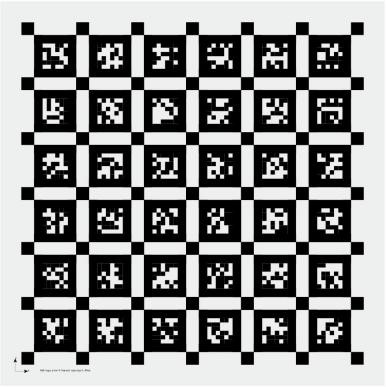
\includegraphics[height=6cm]{figures/april_board}
        \captionof{figure}{April Board上的二维码和棋盘格图案}
        \label{fig:april_board}
    \end{minipage}%
    \begin{minipage}{0.5\textwidth}
        \centering
        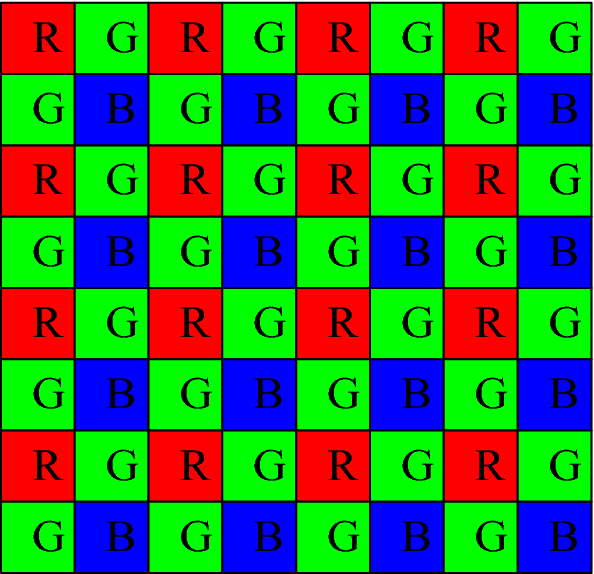
\includegraphics[height=6cm]{figures/bayer}
        \captionof{figure}{Bayer格式照片示意图}
        \label{fig:bayer}
    \end{minipage}%
\end{figure}

本方案中使用的标定物体为April Board,即印有二维码和棋盘格组成的图案的标定板,如图\ref{fig:april_board}所示。
该标定板的尺寸为$800 \times 800$毫米,每个二维码的边长为$88$毫米。
该图案中棋盘格的十字角点可由算法精确完成亚像素级定位,而密集的二维码则便于在不同照片中便捷地匹配角点。
其采用了玻璃基板,以保证标定板的刚性和平整度;
同时采用了氧化铝表面,使标定板表面无明显镜面反射光斑,确保标定板在不同光照条件下的可靠性。

在拍摄标定物体时,需要注意保持相机处于手动对焦模式,关闭光学防抖,以防止其内外参意外发生变化。
并使用前述(第\ref{sec:passive_sync}节)被动相机同步装置同时触发所有相机进行拍摄。转动标定板,重复触发快门15-20次。

\paragraph{相机标定优化目标}
\def\cornerpix{\mathbf{o}}
\def\cornerboard{\mathbf{w}}
本方案中的相机标定算法接收照片中的特征点坐标作为输入,求解上述相机模型中的参数$\camparam$。
正式地,假设共触发了$M$次快门,标定板中共有$K=144$个角点,算法的输入包括第$i$个相机在第$j$次触发快门时拍摄的第$k$个角点($j = 1,2,\cdots,M$、$k = 1,2,\cdots,K$)在像素坐标系中的坐标$\cornerpix_{i,j,k}\in \mathbb{R}^2$;
以及角点在标定板坐标系中的坐标$\cornerboard_k\in \mathbb{R}^3$。
由于每次触发快门时标定板都由人工转动,因此其在世界坐标系中的位置也是未知的,故将第$j$次快门时标定板坐标系到世界坐标系的刚体变换$T_{j}(\cdot)\in \mathrm{SE(3)}$也做为未知量。
其中固定$T_{1}$为幺元,即$T_{1}(X) = X$,以确定世界坐标系的位置。
则本文中的相机标定问题可以表示为以下最小二乘优化问题:
\begin{equation}
    \label{eq:calib_opt}
    \argmin_{\camparam,T} \sum_{i,j,k} \left\| \cornerpix_{i,j,k} - \pi\left(\camparam_i, T_j(\cornerboard_k)\right) \right\|_2^2
    \text{。}
\end{equation}
为实现该目标,首先需要在每张照片中识别角点,并以亚像素级精度精确定位其坐标$\cornerpix_{i,j,k}$。
本节后续将介绍角点的识别、精确定位,模型初始化及上述优化问题的具体求解方法。

\paragraph{角点识别}为识别标定板中可供拟合的角点,本文首先识别照片中的二维码,并将二维码的四个角作为角点的候选点。
本文所用标定板上的二维码为AprilTag,本文实现的识别算法也是基于其开源的方法\cite{AprilTag}。
该算法是一个自下而上的算法,它首先从照片中识别直线段,然后将直线段组合成四边形,最后试图将四边形区域识别为二维码。得益于二维码的纠错功能,虽然该方法召回率稍低,但查准率非常高。同时二维码中存储的信息可用于角点在不同照片中的匹配。

本文所实现的版本的输入为相机拍摄的,原始Bayer格式的照片,该照片是单通道图像,其中RGB像素排列如图\ref{fig:bayer}所示,每$2\times 2$个像素中包括一个红色像素、两个绿色像素和一个蓝色像素。每种像素的传感器前带有滤光片,仅允许特定波长的光被传感器捕获。因此,Bayer格式的照片中,每个像素的值即为该像素对应的颜色通道的光照强度。
为了减少冗余的数据处理流程,并保持全流程的可解释性以准确控制误差,本方案直接使用了原始照片,而没有使用常见的相机后处理后输出的RGB格式图像。

由于我们所拍摄的照片分辨率远超二维码识别所需,因此本文先对照片进行降采样。
其具体方法是,首先在每4个像素中仅取一个绿色像素,以排除颜色对二维码识别的影响;
再进行5倍平均池化,即最终降采样后的图像长宽为原图的$1/10$。
以此降低算法耗时并大大降低照片中的噪声等级,提升算法的鲁棒性。
在低分辨率的图像上完成二维码识别后,二维码的四个角的坐标将被重新映射回完整分辨率的像素坐标,以初始化后续的精确定位步骤。

% 本文使用的相机拍摄的原始照片分辨率高,可达$5472\times 3648$;
% 且宽容度高,其量化后的亮度可达约13000级,相比普通JPG照片仅有256级。
% 因此,本文在\cite{AprilTag}的基础上,设计了尺度、亮度无关的直线段识别算法,使其更加鲁棒,并减少算法超参数调节的麻烦。
% \TODO{尺度、亮度无关的直线段识别算法}

\paragraph{角点精确定位}在上一步识别出角点后,该步骤依据角点周围的像素值,获取这些角点尽可能精确的像素坐标$\cornerpix_{i,j,k}$,以保证标定的精度。
该步骤的难点在于,算法需要对失焦造成的模糊、成像过程中的噪声等因素足够鲁棒,并达到亚像素级的精度。
本文采用的算法为\citet{ROCHADE}提出的精确角点定位算法,其基本思想为:
使用一个二维多项式函数对角点周围的像素进行拟合,然后以该多项式函数的鞍点作为该角点的精确像素坐标。

具体地,本文首先需要从照片原始数据获取单通道灰度图。
该灰度图在标定板区域的每个像素值应表征标定板表面反射的总光强,而不与颜色有关。
为此,需要对红色、蓝色像素值进行缩放,使其与绿色像素匹配(相当于相机的白平衡操作),其缩放系数与环境光照、标定板材质等有关。
本文假设标定板任意位置反射的光线的波长分布是均匀的。
因此,本文首先对上一步求得的二维码区域求凸包,以定位照片中的标定板,并调整缩放系数以使该区域中不同颜色像素的均值相等。
然后,对该图使用半径为$r$的圆锥形kernel进行滤波,以使像素值平滑,从而能更好地被多项式函数拟合。
最后,以角点的当前估计位置为中心,使用二阶二维多项式函数对周围的$2r+1 \times 2r+1$个像素进行最小二乘拟合:
\begin{equation}
    \label{eq:poly}
    \hat{a} = \argmin_{a} \sum_{x,y} \left(\bar{I}(x, y) - (a_0 x^2 + a_1 y^2 + a_2 xy + a_3 x + a_4 y + a_5)\right)^2\text{。}
\end{equation}
在实现上,本方案直接使用解析公式求解该线性最小二乘问题。并求该二维多项式函数的鞍点作为该角点新的估计位置:
\begin{equation}
    \label{eq:subpixel}
    \begin{cases}
        x' &= -\dfrac{\hat{a}_2 \hat{a}_4 - 2 \hat{a}_1 \hat{a}_3}{\Delta} \\
        y' &= -\dfrac{\hat{a}_2 \hat{a}_3 - 2 \hat{a}_0 \hat{a}_4}{\Delta}
    \end{cases},\quad
    \Delta = 4 \hat{a}_0 \hat{a}_1 - \hat{a}_2^2
    \text{,}
\end{equation}
并如此迭代,直到角点的估计位置收敛,该收敛的位置即为$\cornerpix$。
在此过程中,若估计位置超出了图像范围,或$\Delta < 0$,则将该角点排除。
$\Delta < 0$的原因通常是该角点被其他物体遮挡,或者受到其他物体投下的阴影影响。

\def\cornerincode{\hat{\cornerpix}}
在该算法中,$r$的选取可能对结果产生较大影响。较大的$r$将能利用照片中更多像素的信息,从而对噪声更加鲁棒,但也不能过大,否则周边的二维码,或相邻的其他角点等无关信息将影响拟合结果。为此,本文依据上一步识别到的二维码的尺寸以自适应地选择$r$。令$\cornerincode_{i,j}$为照片中第$i$个二维码的第$j$个角点的估计位置,$j\in\{0,1,2,3\}$,以顺时针方向排列,则$r$的选取为:
\begin{equation}
    \label{eq:r}
    \begin{aligned}
        l_{i,\textrm{edge}} & = \min_j\left(\|\cornerincode_{i,j} - \cornerincode_{i,j+1\bmod 4}\|\right)\text{,} \\
        l_{i,\textrm{diag}} & = \min\left(\|\cornerincode_{i,0} - \cornerincode_{i,2}\|, \|\cornerincode_{i,1} - \cornerincode_{i,3}\|\right)\text{,} \\
        r & = \min_i\left\{0.07 l_{i,\textrm{edge}}, 0.05 l_{i,\textrm{diag}}\right\}\text{。}
    \end{aligned}
\end{equation}

\paragraph{多相机内参标定与外参传递}
在第一阶段,本文将对每台相机分别进行标定,获得各相机的内参初始化值
并估计标定版在每次触发快门时与各台相机的相对位置。
具体地,本文依据相机和镜头厂商提供的传感器尺寸、图像分辨率、镜头焦距初始化相机内参$f$、$c$。
然后调用OpenCV中单台相机标定的算法,使用PnP算法求解标定板在每次触发快门时与相机的相对位置$T_{i,j}$;
并使用Levenberg-Marquardt算法对这些参数进行调整。

由于不同相机的同一次快门的触发是严格同步的,因此可以认为若不同相机在同一次快门的触发时,拍摄到的标定板在世界坐标系中的位置是相同的。
据此可将每台相机,以及每次快门触发作为节点,构建二部图,图中的边表示该相机在该次快门中拍摄到了标定板。
若该二部图是连通图,则可迭代地将所有相机、所有快门触发中的标定板的位置传递到世界坐标系中,
如算法\ref{alg:calib_init}所示。
并最终获得$\delta$和$T$中所有参数的初始化值。

\begin{algorithm}[t]
    \caption{外参传递}
    \label{alg:calib_init}
    \begin{algorithmic}[1]
        \Require 连通二部图$(V,E)$;第$j$次快门时标定版坐标系到相机$i$坐标系的刚体变换$\hat{T}_{i,j}\in SE(3),(i,j)\in E$
        \Procedure{外参传递}{$V,E,\hat{T}_{i,j}$}
            \State $C \gets \emptyset$\Comment{已传递的相机集合}
            \State $T_{1} \gets \mathbf{I}$\Comment{以第$1$次快门时标定版坐标系作为世界坐标系}
            \State $S \gets \{1\}$\Comment{已传递的快门触发集合}

            \While{$C \cup S \neq V$}
                \State $i \gets \forall i\in V| i\notin C, \exists j\in S| (i,j)\in E$
                    \Comment{选择与已知位置的标定板相邻的相机}
                \State $U_{i} \gets T_{j}\hat{T}_{i,j}^{-1}$
                    \Comment{相机$i$到世界坐标系的变换}
                \State $C \gets C \cup \{i\}$
                \ForAll{$j | (i,j)\in E, j\notin S$}
                    \State $T_{j} \gets U_{i}\hat{T}_{i,j}$
                        \Comment{第$j$次快门时标定版到世界坐标系的变换}
                \EndFor
                \State $S \gets S \cup \{j\in V| (i,j)\in E\}$
            \EndWhile
            \State \Return $U, T$
        \EndProcedure
    \end{algorithmic}
\end{algorithm}

\paragraph{集束调整}在第二阶段,本文将对所有相机进行集束调整,即直接使用公式\eqref{eq:calib_opt}中的目标函数,在上一阶段的初始化值的基础上,同时优化模型中的所有参数。
具体地,本文使用了Levenberg-Marquardt算法\cite{lm},对目标函数进行优化求解。
并手动实现了公式\eqref{eq:calib_opt}的雅克比矩阵的解析求解算法,以提升算法的速度和收敛精度。

然后,排除掉误差较大的角点,再次重复上述优化过程,并如此迭代数次,每次使用更严格的误差阈值进行排除。
这些误差较大的角点通常是由于角点定位不准确造成的,因此,将其排除后可以提高标定的精度。
该优化过程最终得到的相机参数$\camparam$即为所求的最终的相机标定结果。


\section{基于反射球的光源标定和HDRI合成}

\section{主动相机/闪光灯同步}

主动相机同步装置有单片机等实时控制系统控制,能独立控制每台相机、闪光灯触发延迟,最多24个通道。可用于快速抓拍不同闪光灯照明下的照片

\paragraph{主动同步装置硬件设计}

\paragraph{主动同步装置软件设计}

\paragraph{滚动快门原理}

\paragraph{闪光灯触发延迟快速标定方法}

\section{照片拍摄和整理流程}

\paragraph{同步装置连接与设定}

\paragraph{拍摄采集对象}

\paragraph{相机、光源标定数据采集}

\paragraph{照片拷贝和整理}

\section{初步验证}

作为该实验平台实用性的初步验证,本文利用该平台采集的数据使用传统的计算机视觉方法尝试重建人脸模型。

本文首先使用Colmap完成人脸的稀疏以及稠密点云重建。\TODO{参数调整}

然后,本文使用FlameFitting工具,将FLAME 3D模型配准到稠密点云上,得到初步的人脸几何形状。

然而,该配准的效果并不理想。因此本文使用Blender同时导入点云和几何形状,并手动调整模型顶点位置以完成更精确的配准。

最后,本文通过Unwrap方法,将照片映射到UV空间,每个视角获得一张纹理贴图,再将这些纹理贴图通过以下方式进行融合,最终获得一个带纹理的3D人脸模型。

\TODO{融合方式公式}

\TODO{结果图}

\section{后续工作}

然而,这种方法仅仅是对该平台采集的数据的初步利用,仅发挥了该平台的一小部分价值。
该平台的设计目标是用于运行可微分渲染算法,后续的研究者们将能利用该平台开展诸多基于可微分渲染的研究,例如:
\begin{itemize}
\item 在传统计算机视觉重建的几何形状的基础上,利用可微分渲染算法,实现符合基于物理的渲染(PBR)流程的人脸材质,包括粗糙度、次表面散射等参数。
\item 利用所采集到的HDRI光源信息,基于分离求和近似(split sum approximation)的可微分光栅化渲染算法,直接端到端地同时估计人脸的几何结构和材质。
\item 利用光线追踪方法,进一步考虑全局光照,以估计更加准确的材质。
\item 将本系统所使用的消费级微单相机更换为工业相机,以实现视频帧同步,可将该实验平台扩展为采集人脸动态表情数据。
\end{itemize}

\chapter{结论与展望}
\label{chap:conclusion}

\backmatter
\bibliography{main}

\chapter{致谢}

\end{document}
